\section*{Suchen}
\subsection*{Sequenzielle Suche}
\begin{minted}{java}
int search(int[] arr, int x) {
    for(int i = 0; i < arr.length; i++) 
        if(arr[i] == x) 
            return i; 
    return -1; 
}
\end{minted}
\subsection*{Sequenzielle Suche mit Wächter}
\begin{minted}{java}
boolean search(int[] data, int value){
    int last = arr[n - 1];  
    arr[n - 1] = x;  
    int i = 0;  
    while (arr[i] != x)  
        i++;  
    arr[n - 1] = last;
    return (i < n - 1) || (x == arr[n - 1]);
}
\end{minted}
\subsection*{Binäre Suche}
\begin{minted}{java}
int binSearch(int[] data, int value){
  int l = -1, h = data.length + 1;
  while(l+1 != h){
    int m = (l + h) \ 2;
    if(data[m] < value)
      l = m;
    else if(data[m] > value)
      h = m;
    else
      return m;
  }
  return -1;
}
\end{minted}
\columnbreak
\subsection*{Binäre Suche Speziell}
\resizebox{\columnwidth}{!}{%
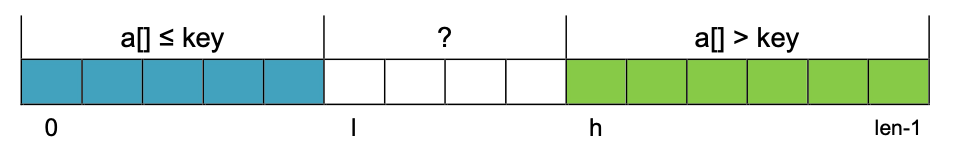
\includegraphics[width=10cm]{images/binsuche}}
\begin{minted}{java}
int binSearch1(int[] data, int key) {
  int l = 0, h = data.length;
  while (l != h) {
    int m = (l + h) / 2;
    if(data[m]<=key)l=m+1;
    else h=m;
  }
  return l - 1; 
}
\end{minted}
\subsection*{Binäre Suche für Objekte}
\begin{minted}{java}
<T extends Comparable<? super T>> int binSearch(T[] data, 
T value) {
	int l = -1, h = data.length;
	while (l + 1 != h) {
		int m = (l + h) >>> 1;
		int c = data[m].compareTo(value); 
		if (c < 0) l = m;
		else if (c > 0) h = m;
		else return m;
	}
	return NOT_FOUND; 
}
\end{minted}
\subsection*{Max Sub Array}
\begin{minted}{java}
int maxSub(int[] data) {
  int max = 0, cur = 0;
  for (int end = 0; end < data.length; end++) {
    cur = cur > 0 ? cur + data[end] : data[end];
	if (cur > max) max = cur;
  }
  return max;
}
\end{minted}

